\documentclass{beamer}
\usepackage{amsmath}
\usepackage{amsfonts}
\usepackage{amssymb}
\usepackage{graphicx}
%\usepackage{enumerate}
\usepackage{stmaryrd}
%\usepackage{wrapfig}
\usepackage{csquotes}
\usepackage{listings}
\usepackage{unicode-math}
\usepackage{polyglossia}

\setmainlanguage{english}

\usetheme{Warsaw}
\newtheorem{theo}[theorem]{Théorème}
\title{The Li(sp)Monade processor}
\author[ENS Ulm]{Nguyễn Lê Thành Dũng \and Thomas Bourgeat}
\date{January 28, 2014}

\begin{document}

\begin{frame}
  \titlepage
\end{frame}

\begin{frame}{Plan}
  \tableofcontents
\end{frame}

\section{Introduction}

\begin{frame}{Objectives}
\begin{itemize}
\item Implement a processor suited for functional languages.
\begin{itemize}
\item Native support for closures, function applications, \dots
\item Hardware level allocator.
\end{itemize}
\item Peter Landin's SECD, the Krivine machine, \dots
\item Our choice: the \emph{Lisp machine} family.  
\end{itemize}
\end{frame}

\begin{frame}{A little bit of history on Lisp machine}
\begin{itemize}
\item Studied in 70's and 80's in the MIT AI Lab.
\item Highly influential Lisp hacker culture e.g Emacs.
\item Lisp machine for industrial applications : CADR, \dots
\item Experimental architectures : SIMPLE and SCHEME-79.
\end{itemize}
\end{frame}

\begin{frame}{Main originalities}
\begin{itemize}
\item An non-linear assembly language!
\begin{itemize}
\item Machine code consists of a syntax tree instead of a list of instructions
\end{itemize}
\item Homoiconicity
\item Very close to the structure of a Lisp program.
\begin{itemize}
\item Compilation is trivial
\end{itemize}
\end{itemize}
\end{frame}

\begin{frame}{Demo}
\begin{itemize}
\item A clock executed on the Li(sp)Monade processor.
\pause
\item Now, let us see the source code.
\end{itemize}
\end{frame}

\begin{frame}[fragile]
\frametitle{Source}
\begin{lstlisting}[language=Lisp,basicstyle=\scriptsize]
(defun main ()
  (count-hours 18))

(defun count-hours (hr)
  (print-hour hr) 
  (count-minutes 0)
  (let ((new-hr (+1 hr)))
    (if (>=24? new-hr)
        (synchronize (count-hours 0)) 
        (synchronize (count-hours new-hr)))))

(defun count-minutes (min)
  (print-minute min)
  (count-seconds 0)
  (let ((new-min (+1 min)))
    (if (>=60? new-min)
        ()  
        (synchronize (count-minutes new-min)))))
\end{lstlisting}

\end{frame}

\section{The S-Code assembly language.}

\begin{frame}[fragile]
\frametitle{The answer to the universe (using Lisp)}
\begin{lstlisting}[language=Lisp]
(defun answer () 
  (print (+1 41)))
\end{lstlisting}
\end{frame}

\begin{frame}{The answer to the universe (using S-Code)}
\begin{figure}[h]
\center
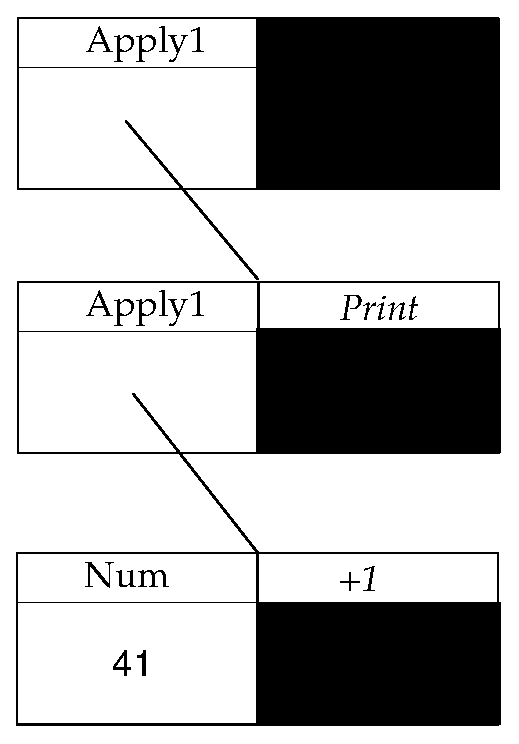
\includegraphics[scale=0.5]{answerscode.eps}
\end{figure}
\end{frame}

\begin{frame}{An abstract execution environment.}
\begin{itemize}
\item 5 registers (+Null register): Expr, Value, Env, Args, Stack with the
\emph{mov}
operations.
\item A memory system which provides primitives like fetchCar, allocCons \dots 
\end{itemize}
\end{frame}


\begin{frame}{How to evaluate a function application}
\begin{itemize}
\item Save the environment (Local variables)
\item Launch the evaluation on the argument
\item Put the value in the list of arguments: Args register.
\item Save the args list
\item Restore the environment
\item Evaluate the function
\end{itemize}
\end{frame}

\begin{frame}[fragile]
\frametitle{Sample of microprogram}
\begin{itemize}
\item Apply1:
\begin{lstlisting}
push Env 
pushWithReturn RApplyOne Expr
fetchCar Expr Expr
dispatchEval (*Dispatch on expr*) 
\end{lstlisting}
\item Num:
\begin{lstlisting}
Value:=Expr
dispatchReturn (*Dispatch on stack*)
\end{lstlisting}
\end{itemize}
\end{frame}

\begin{frame}{Hardware implementation}
\begin{itemize}
\item The microinstructions are easier to execute than instructions.  
\item The crux of the problem is to trigger several microinstructions from one
instruction.  
\end{itemize}
\end{frame}


\begin{frame}{Hardware implementation(2)}
\begin{figure}[h]
\center
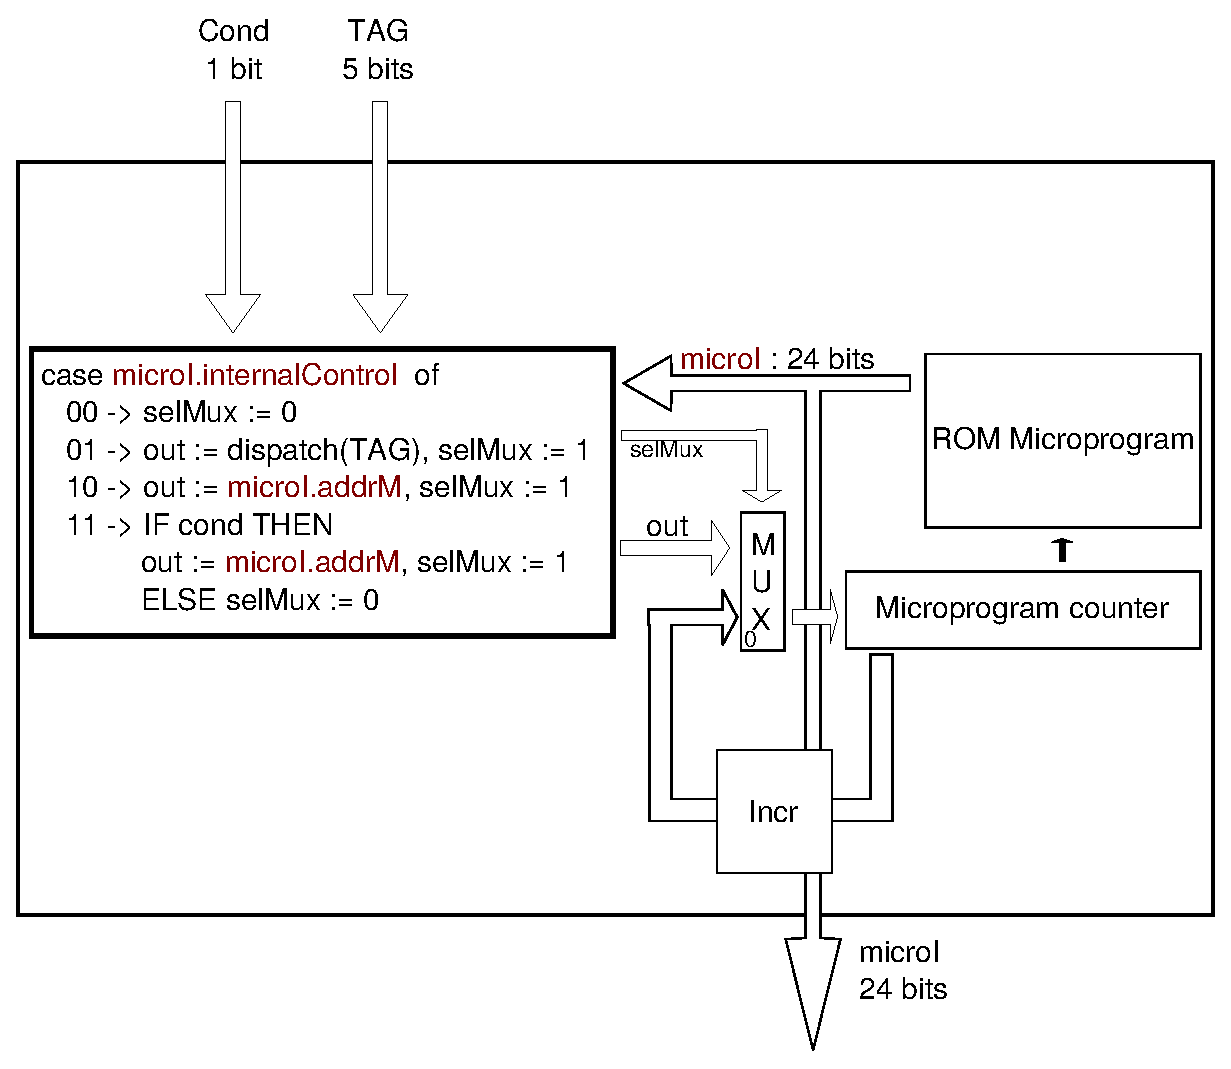
\includegraphics[scale=0.40]{control.eps}
\end{figure}
\end{frame}

\section{Functional units of the processor}
\begin{frame}{ALU}
\begin{figure}[h]
\center
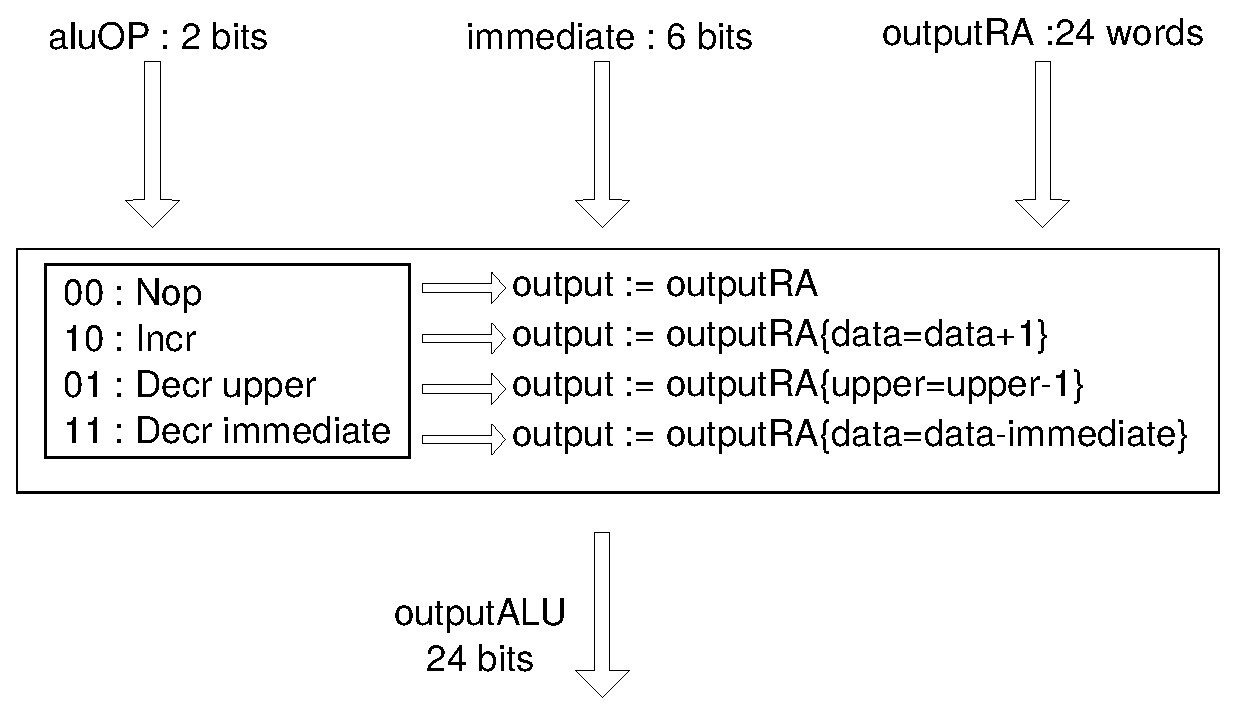
\includegraphics[scale=0.40]{ALU.eps}
\end{figure}
\pause
\begin{itemize}
\item Nothing to see here.
\end{itemize}
\end{frame}

\begin{frame}{Memory system}
\begin{itemize}
\item Objective: Provide a hardware abstraction layer over memory
\item Primitives implemented:
\begin{itemize}
\item Allocating a cons cell
\item Extracting the first and the second half of a cell. i.e dereferencing
pointers.
\end{itemize}   
\end{itemize}
\end{frame}

\begin{frame}{Memory: How it's done}
\begin{figure}[h]
\center
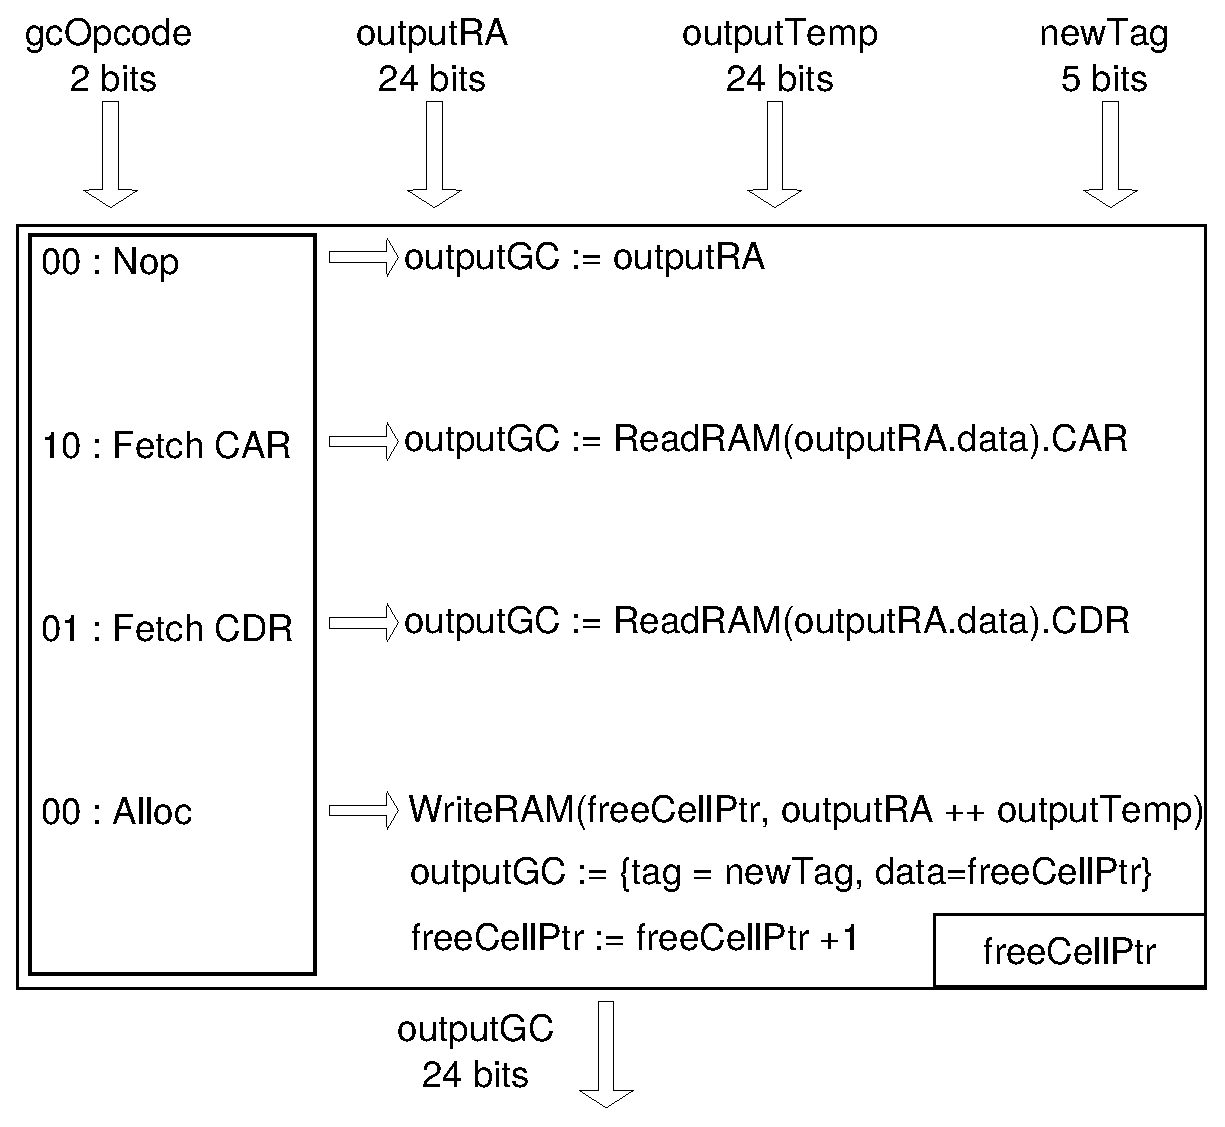
\includegraphics[scale=0.40]{GC.eps}
\end{figure}
\end{frame}


\section{Time management}

\begin{frame}{Time management at all levels}
\begin{itemize}
\item \emph{Lisp/S-code:} A \enquote{synchronize} instruction which wait for the next
system second to resume the computation.
\item \emph{Harware:} A microinstruction which results in an output signal from
the circuit.
\item \emph{Simulator:} Reacts to the signal by suspending the computation. 
\end{itemize}
\end{frame}

\end{document}
